% !TeX spellcheck = id_ID
\documentclass[a4paper,12pt]{article}
\usepackage[indonesian]{babel}
\usepackage{graphicx}
\usepackage{multirow}
\usepackage{enumitem}
\usepackage{listings}
\usepackage{wrapfig}
\usepackage[T1]{fontenc}
\usepackage{inconsolata}
\usepackage{lipsum}
\usepackage{adjustbox}


\usepackage{color}
\usepackage[table]{xcolor}
\definecolor{mygreen}{rgb}{0,0.6,0}
\definecolor{mygray}{rgb}{0.5,0.5,0.5}
\definecolor{mymauve}{rgb}{0.58,0,0.82}
\lstset{%
    language=java,
    showstringspaces=false,          % Prevent tex replacing space to bracket in code
    frame=single,                    % Set frame around code
    backgroundcolor=\color{white},   % choose the background color
    basicstyle=\footnotesize,        % size of fonts used for the code
    breaklines=true,                 % automatic line breaking only at whitespace
    captionpos=b,                    % sets the caption-position to bottom
    commentstyle=\color{mygreen},    % comment style
    escapeinside={\%*}{*)},          % if you want to add LaTeX within your code
    keywordstyle=\color{blue},       % keyword style
    stringstyle=\color{mymauve},     % string literal style
}

\graphicspath{ {./img/} }
\begin{document}
\title{ {\Large Laporan Praktikum}\\ Algoritma dan Pemrograman Lanjut\\{\Large Pertemuan 3}}

\author{Aldzikri Dwijayanto Prathama 
	\\195410189
	\\Informatika}
\makeatletter
\begin{titlepage}
	\begin{center}
		{\huge \bfseries \@title }\\[14ex]
		
\includegraphics[scale=.8]{logo}\\[4ex]
		{\large \@author}\\[12ex]
		{\large \bfseries {SEKOLAH TINGGI MANAJEMEN INFORMATIKA DAN KOMPUTER
				AKAKOM YOGYAKARTA}}
	\end{center}


%{\large \@date} 
\end{titlepage}
\makeatother
%\maketitle
\newpage
\tableofcontents
\newpage

\section{Tujuan}
\paragraph{}
Mahasiswa dapat :
\begin{enumerate}
    \item Menjelaskan konsep array 1dimensi
    \item Menjelaskan perbedaan array dengan data
    \item Merencanakan struktur data dalam bentuk array 1 dimensi
    \item Mengaplikasikan array
\end{enumerate}

\section{Teori}
\paragraph{}
Array adalah sebuah variabel yang bisa menyimpan banyak data dalam
satu variabel.
Array menggunakan indeks untuk memudahkan akses terhadap data
yang disimpannya.
Indeks array selalu dimulai dari 0 dan perlu diketahui juga, indeks tidak
selalu dalam bentuk angka. Bisa juga karakter atau teks.

\newpage

\section{Pembahasan}
\subsection{Praktik}
\subsubsection{Praktik 1}
\begin{lstlisting}
public class Array1
{
    public static void main (String[] args)
    {
        //array 1 dimensi
        String[] nama = new String[5];
        nama[0] = "Jono";
        nama[1] = "Joni";
        nama[2] = "Jini";
        nama[3] = "Jeni";
        nama[4] = "Juni";
        //menampilkan array menggunakan for
        for (int i=0; i<nama.length; i++)
        System.out.println(nama[i]);
    }
}
\end{lstlisting}
Program tersebut memiliki array 1 dimensi. Array dideklarasikan dengan String[] nama, itu berarti array tersebut terdiri dari tipe data string, lalu panjangnya didefinisikan dengan new String[5]
yang berarti array tersebut memiliki panjang data sejumlah 5. Setelah panjangnya ditentukan array diisi. Karena indeks array dihitung dari 0, maka indeks pertama yang diisi adalah indeks 0 
sampai indeks 4. Setelah itu program akan mengeprint isi dari array, dengan menggunakan perulangan for. Init diberi nilai 0, karena array dimulai dari 0. Kondisinya init < panjang array.\\
Sehingga jika dijalankan program akan menghasilkan output seperti berikut:\\
\begin{center}
    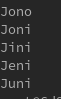
\includegraphics[scale=.7]{1.png}
\end{center}

\subsubsection{Praktik 2}
\begin{lstlisting}
public class Array1b {
    public static void main(String[] args) {
        //array 1 dimensi
        String[] nama = {"Jono","Joni","Jini","Jeni","Juni"};
        //menampilkan array menggunakan foreach
        for (String name:nama)
            System.out.println(name);
    }
}
\end{lstlisting}
Jika isi dari array dideklarasikan di dalam program maka kita bisa langsung mengisinya tanpa menentukan panjang array, dan menyertakan indeks ke berapa data tersebut akan diisikan. 
Data akan diisikan ke dalam indeks array sesuai urutannya.
Selain itu kita juga bisa mengeprint isi array dengan for each, jadi perulangan akan akan mengulang sesuai dengan jumlah data di dalam array, kita tidak perlu menentukan init dan kondisi 
untuk for tersebut.\\
Sehingga jika program dijalankan maka akan menghasilkan output berikut:\\
\begin{center}
    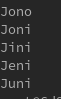
\includegraphics[scale=.7]{1.png}
\end{center}

\subsubsection{Praktik 3}
Selain string array juga bisa menyimpan tipe data lain, untuk string dengan tipe data integer dapat dideklarasikan sama seperti sebelumnya
\begin{lstlisting}
public class Array1c {
    public static void main(String[] args) {
        String[] nama = {"Jono","Joni","Jini","Jeni","Juni"};
        int[]umur={25, 30, 55, 35, 40};
        System.out.println("Nama\tUmur");
        //menampilkan array
        for (int i=0; i<nama.length; i++)
            System.out.println(nama[i]+"\t " +umur[i]);
    }
}
\end{lstlisting}
Karena array nama dan umur memiliki panjang data yang sama, maka kondisi untuk for dapat menggunakan panjang dari array nama.\\
Output dari program tersebut seperti berikut:\\
\begin{center}
    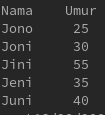
\includegraphics[scale=.7]{2.png}
\end{center}

\subsubsection{Praktik 4}
\begin{lstlisting}
import java.util.Scanner;
public class ArrayInputUser {
    public static void main(String[] args) {
        int bilangan[] = new int[4];
        int i,j;
        Scanner input = new Scanner(System.in);
        for (i=0;i<=3;i++) {
            System.out.print("Silahkan masukan bilangan : ");
            bilangan[i] = input.nextInt();
        }
        //untuk menampilkan array
        for (j=0;j<=3;j++) {
            System.out.println("Bilangan yang anda masukkan" +" "+
            bilangan[j]);
        }
    }
}
\end{lstlisting}
Program diatas mampu memasukkan nilai yang diberi oleh user ke array pada saat program dijalankan. Dengan menggunakan perulangan for, maka program akan memasukkan input ke array ke 
dalam array ke dalam indeks yang sesuai dengan jumlah perulangan. Maka jika program dijalankan akan seperti berikut:\\
\begin{center}
    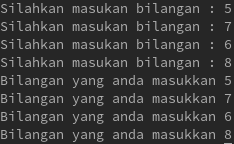
\includegraphics[scale=.7]{3.png}
\end{center}

\newpage

\subsubsection{Praktik 5}
\begin{lstlisting}
import java.util.Scanner;
public class Larik2{
    public static void main(String args[]){
        Scanner masuk = new Scanner(System.in);
        float nilai[]= new float[5];
        float total,rata;
        System.out.println("Masukan 5 buat data nilai");
        for (int i = 0; i < 5; i++)
        {
            System.out.print( (i + 1 )+" : ");
            nilai[i]=masuk.nextFloat();
        }
        System.out.println("Data nilai yang dimasukan");
        for (int i = 0; i < 5; i++)
            System.out.println(nilai[i]);
        total = 0;
        for (int i = 0; i < 5; i++)
            total = total + nilai[i];
        rata = total/5;
        System.out.println("Total data = "+total);
        System.out.println("Rata-rata = "+rata);
    }
}
\end{lstlisting}
Program tersebut akan menjumlahkan semua data yang ada di array. Dengan menggunakan perulangan for dan pernytaan total = total + nilai[i] maka program akan menjumlahkan semua data yang ada 
didalam array nilai. Setelah itu untuk menghitung rata-rata maka variabel total dibagi dengan 5.
\begin{center}
    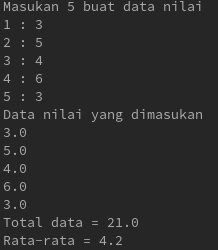
\includegraphics[scale=.7]{4.png}
\end{center}

\newpage

\subsubsection{Praktik 6}
\begin{lstlisting}
import java.util.Scanner;
public class Larik2a{
    public static void main(String args[]){
        Scanner masuk = new Scanner(System.in);
        float nilai[]= new float[5];
        float total,rata,besar,kecil;
        System.out.println("Masukan 5 buat data nilai");
        for (int i = 0; i < 5; i++)
        {
            System.out.print( (i + 1 )+" : ");
            nilai[i]=masuk.nextFloat();
        }
        System.out.println("Data nilai yang dimasukan");
        for (int i = 0; i < 5; i++)
            System.out.println(nilai[i]);
        total = 0;
        for (int i = 0; i < 5; i++)
            total = total + nilai[i];
        rata = total/5;
        besar=nilai[0];
        for (int i = 1; i < 5; i++){
            if(besar < nilai[i]){
                besar = nilai[i];
            }
        }
        kecil=nilai[0];
        for (int i = 1; i < 5; i++){
            if(kecil > nilai[i]){
                kecil = nilai[i];
            }
        }
        System.out.println("Nilai terkecil = "+kecil);
        System.out.println("Nilai terbesar = "+besar);
        System.out.println("Total data = "+total);
        System.out.println("Rata-rata = "+rata);
    }
}
\end{lstlisting}
Program tersebut merupakan program dari praktik sebelumnya yang dimodifikasi dengan menambahkan perulangan yang memiliki pernyataan seleksi. Seleksi tersebut akan membandingkan data dalam 
array untuk mencari nilai terbesar dan terkecil, lalu menyimpannya ke dalam variabel besar untuk nilai terbesar, dan kecil untuk variabel terkecil.
\begin{center}
    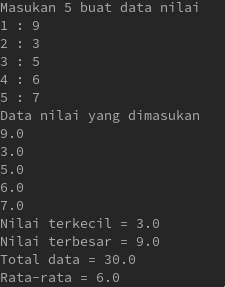
\includegraphics[scale=.7]{5.png}
\end{center}

\subsection{Latihan}
\subsubsection{Latihan 1}
\begin{lstlisting}
import java.util.Scanner;
public class Biodata_Mhs {
    public static void main(String[] args){
        Scanner input = new Scanner(System.in);
        String nama, nim, jenisKelamin, alamat, nope, def="Masukan ";
        System.out.println("================================");
        System.out.println("| INPUT BIODATA MAHASISWA |");
        System.out.println("================================");
        System.out.print(def + "Nama \t\t: " );
        nama = input.nextLine();
        System.out.print(def + "NIM \t\t: " );
        nim = input.nextLine();
        System.out.print(def + "Jenis Kelamin \t: " );
        jenisKelamin = input.nextLine();
        System.out.print(def + "Alamat \t\t: " );
        alamat = input.nextLine();
        System.out.print(def + "Nomor Handphone\t: " );
        nope = input.nextLine();
        System.out.println("");
        System.out.println("+------------------------------+");
        System.out.println("| Data Biodata Mahasiswa |");
        System.out.println("+------------------------------+");
        System.out.println("| Nama\t\t: " + nama);
        System.out.println("| NIM\t\t: " + nim);
        System.out.println("| Jenis Kelamin\t: " + jenisKelamin);
        System.out.println("| Alamat\t: " + alamat);
        System.out.println("| Nomor HP\t: " + nope);
        System.out.println("+-------------------------------+");
    }
}
\end{lstlisting}
Program tersebut merupakan program yang akan mnampilkan biodata mahasiswa. Saat dijalankan program akan menampilkan biodata mahasiswa yang sebelumnya dimasukkan 
oleh user yang disimpan ke dalam variabel biasa, bukan array. Jika dijalankan akan maka program akan menghasilkan output seperti berikut:\\
\begin{center}
    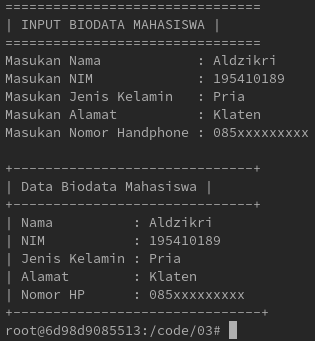
\includegraphics[scale=.7]{6.png}
\end{center}

\subsubsection{Latihan 2}
\begin{lstlisting}
import java.util.Scanner;
public class Latihan {
    public static void main(String[] args) {
        Scanner input = new Scanner(System.in);
        String jur;
        String nama;
        String nim;
        int batas;
        System.out.println("==================================");
        System.out.println("Menghitung Nilai Mahasiswa");
        System.out.println("==================================");
        System.out.print("Masukan Jumlah Mata Kuliah: ");
        batas = input.nextInt();
        input.nextLine();
        String[] matkul = new String[batas];
        String[] grade = new String[batas];
        float[] uas= new float[batas];
        float[] uts= new float[batas];
        float[] rata= new float[batas];
        float[] jumlah= new float[batas];
        System.out.println("==================================");
        System.out.print("Nama\t:");
        nama = input.nextLine();
        System.out.print("NIM\t:");
        nim = input.nextLine();
        System.out.print("Jurusan\t:");
        jur = input.nextLine();
        System.out.println("==================================");
        System.out.println();
        for(int i = 0; i < batas; i++){
            int print = i + 1;
            System.out.print("Mata kuliah ke-"+print+" :");
            matkul[i] = input.nextLine();
            System.out.print("Nilai UTS : ");
            uts[i] = input.nextFloat();
            System.out.print("Nilai UAS : ");
            input.nextLine();
            uas[i] = Float.parseFloat(input.nextLine());
            System.out.println();
        }
        input.close();
        for (int i=0; i<batas; i++){
            jumlah[i] = uas[i] + uts[i];
        }
        for (int i=0; i<batas; i++){
            rata[i]=jumlah[i]/2;
        }
        for (int i=0; i<batas; i++){
            if(rata[i] >= 85){
                grade[i] = "A";
            }
            else if(rata[i] >= 75){
                grade[i] = "B";
            }
            else if(rata[i] >= 60){
                grade[i] = "C";
            }
            else if(rata[i] >= 50){
                grade[i] = "D";
            }
            else {
                grade[i] = "E";
            }
        }
        System.out.println("==================================");
        System.out.println("Nama :"+nama+"\tNPM : "+nim);
        System.out.println("==================================");
        System.out.println("Mata Kuliah     Nilai       Grade");
        System.out.println("==================================");
        for (int i=0; i<batas; i++){
            System.out.println(matkul[i] + "\t\t"+rata[i]+"\t\t"+grade[i]);
        }
    }
}
\end{lstlisting}
Program di atas akan menampilkan biodata mahasiswa, dan menghitung nilai berdasarkan nilai yang dimasukkan oleh user. panjang array akan mengikuti nilai dari 
variabel batas. Untuk pemberian grade digunakan seleksi. Jika dijalankan program akan menghasilkan output seperti berikut:\\
\begin{center}
    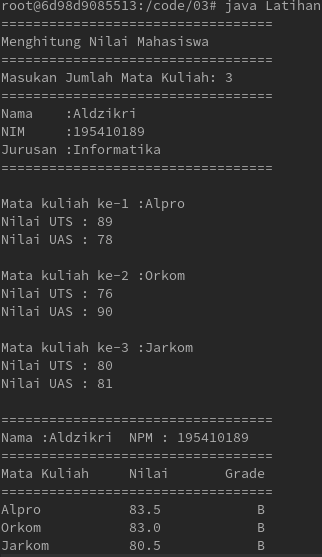
\includegraphics[scale=.7]{7.png}
\end{center}

\subsection{Tugas}
\begin{lstlisting}
import java.util.Scanner;
public class Tugas
{
    public static void main (String[] args) 
    {
        Scanner in = new Scanner(System.in);
        int batas,besar,kecil;
        float jumlah;
        System.out.print("Masukkan panjang data = ");
        batas = in.nextInt();
        int[] nilai = new int[batas];
        for(int i = 0; i < nilai.length; i++)
        {
            int ke = i + 1;
            System.out.print("Masukkan nilai ke-"+ke+" :");
            nilai[i] = in.nextInt();
        }
        in.close();

        jumlah = 0;
        for(int i = 0; i < nilai.length; i++)
        {
            jumlah = jumlah + nilai[i];
        }
        System.out.println("Jumlah = "+jumlah);

        jumlah = jumlah / batas;
        System.out.println("Rata-rata = "+jumlah);

        besar=nilai[0];
        kecil=nilai[0];
        for(int i = 1; i < nilai.length; i++)
        {
            if(besar<nilai[i])
            {
                besar = nilai[i];
            }
            if(kecil>nilai[i])
            {
                kecil = nilai[i];
            }
        }
        System.out.println("Nilai terbesar = "+besar);
        System.out.println("Nilai terkecil = "+kecil);
    }
}
\end{lstlisting}
Program tersebut akan menjumlahkan semua data yang ada di array. Panjang data array tersebut mengikuti nilai yang ada dalam variabel batas. Dengan menggunakan perulangan for dan pernytaan total = total + nilai[i] maka program akan menjumlahkan semua data yang ada 
didalam array nilai. Setelah itu untuk menghitung rata-rata maka variabel total dibagi dengan variabel batas. Lalu terdapat perulangan yang memiliki pernyataan seleksi. Seleksi tersebut akan membandingkan data dalam variabel array. 
\begin{center}
    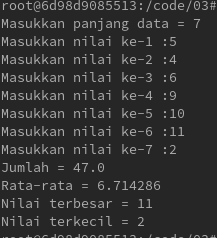
\includegraphics[scale=.7]{8.png}
\end{center}


\newpage
\section{Kesimpulan}
Setelah praktik ini mahasiswa mampu Menjelaskan konsep array 1dimensi dan perbedaan array dengan data, Merencanakan struktur data dalam bentuk array 1 dimensi, serta
Mengaplikasikan array

\end{document}
